% =====================================================================
\section{Asymptotics}\label{sec:asymptotics}
% =====================================================================

Both ends of the real line have clean asymptotics, and the right end
hides a surprise: at infinity the Tahawus function is a square
super-root \emph{shifted by exactly one}. Throughout, $x := \Tah(y)$,
and the starting point is an \emph{exact} identity obtained by taking
logarithms of the defining equation $x^{x} = xy + 1$ and peeling off
$\ln x$:
\begin{equation}\label{eq:master}
    x\ln x \;=\; \ln x + \ln y + \ln\Bigl(1 + \frac{1}{xy}\Bigr)
    \qquad\Longleftrightarrow\qquad
    (x - 1)\ln x \;=\; \ln y + \ln\Bigl(1 + \frac{1}{xy}\Bigr) ,
\end{equation}
the \emph{master identity on the right}. The super square root
$\ssqrt(y) = \ee^{W(\ln y)}$ of \eqref{eq:ssqrt} is the solution of
$x\ln x = \ln y$; the Tahawus function is the solution of
\eqref{eq:master}, which differs from it by the shift $x \mapsto x-1$
in the left factor and by a logarithmically tiny correction on the
right. Both differences push $x$ \emph{up} relative to $\ssqrt(y)$.

\begin{theorem}[asymptotics]\label{thm:asymptotics}
\begin{enumerate}[label=\textup{(\roman*)}, leftmargin=2.4em]
\item \emph{(far left)} As $y \to -\infty$,
\begin{equation}\label{eq:asym-left}
    \ln \Tah(y) \;=\; y - \frac{y^{2}}{2}\,\ee^{y}\bigl(1 + o(1)\bigr),
    \qquad\text{equivalently}\qquad
    \Tah(y) \;=\; \ee^{y} - \frac{y^{2}}{2}\,\ee^{2y}\bigl(1 + o(1)\bigr).
\end{equation}
\item \emph{(far right, plus-one law)} As $y \to +\infty$,
\begin{equation}\label{eq:asym-plusone}
    \Tah(y) \;-\; \ssqrt(y) \;\longrightarrow\; 1 .
\end{equation}
\item \emph{(far right, logarithmic scale)} As $y \to +\infty$,
\begin{equation}\label{eq:asym-right}
    \Tah(y) \;=\; \frac{\ln y}{\ln\ln y}
    \Bigl( 1 + \frac{\ln\ln\ln y}{\ln\ln y} +
    O\Bigl( \bigl(\tfrac{\ln\ln\ln y}{\ln\ln y}\bigr)^{2} \Bigr)
    \Bigr).
\end{equation}
\end{enumerate}
\end{theorem}

\begin{proof}
(i) Expand $f$ at $x = 0^{+}$: with $u := x \ln x \to 0$,
\[
    y \;=\; \frac{\ee^{u} - 1}{x}
    \;=\; \frac{u + \tfrac{u^{2}}{2} + O(u^{3})}{x}
    \;=\; \ln x + \frac{x\ln^{2} x}{2} + O\bigl(x^{2}\ln^{3}x\bigr) .
\]
Since $x \ln^{2} x \to 0$, we get $y - \ln x \to 0$, i.e.\
$\ln x = y + o(1)$ and $x = \ee^{y}(1 + o(1))$. Substituting back,
\[
    y - \ln x \;=\; \frac{x \ln^{2} x}{2}\bigl(1 + o(1)\bigr)
    \;=\; \frac{y^{2}}{2}\,\ee^{y}\bigl(1 + o(1)\bigr),
\]
which is \eqref{eq:asym-left}; the second form follows from
$\exp\bigl(-\tfrac{y^{2}}{2}\ee^{y}(1+o(1))\bigr) =
1 - \tfrac{y^{2}}{2}\ee^{y}(1+o(1))$, legitimate because
$\tfrac{y^{2}}{2}\ee^{y} \to 0$.

(ii) Write $L := \ln y$, let $x_{0} := \ssqrt(y) = \ee^{W(L)}$ (so
$x_{0}\ln x_{0} = L$), and let $\Phi(t) := (t-1)\ln t$, strictly
increasing on $[1, \infty)$. By \eqref{eq:master}, $x =
\Phi^{-1}(L + \varepsilon)$ with
$\varepsilon := \ln\bigl(1 + \tfrac{1}{xy}\bigr) \to 0$, while
$\Phi(x_{0} + 1) - \Phi(x_{1}) = \Phi(x_{0}+1) - L$ where $x_{1} :=
\Phi^{-1}(L)$. Now
\[
    \Phi(x_{0}+1) - L \;=\; x_{0}\ln(x_{0}+1) - x_{0}\ln x_{0}
    \;=\; x_{0}\ln\Bigl(1 + \frac{1}{x_{0}}\Bigr) \;\longrightarrow\; 1,
\]
since $x_{0} \to \infty$. By the mean value theorem there is
$\eta$ between $x_{1}$ and $x_{0}+1$ with
$(x_{0} + 1 - x_{1})\,\Phi'(\eta) = \Phi(x_{0}+1) - L \to 1$; as
$x_{0} \to \infty$ forces $\eta \to \infty$ and
$\Phi'(\eta) = \ln\eta + 1 - \tfrac1\eta \to \infty$, we conclude
$x_{1} - x_{0} \to 1$. Similarly $x - x_{1} = \Phi^{-1}(L+\varepsilon)
- \Phi^{-1}(L)$ lies between $0$ and
$\varepsilon/\Phi'(\xi) \to 0$ (mean value theorem again, with
$\xi \ge x_{1}/2 \to \infty$ for large $y$). Adding,
\[
    \Tah(y) - \ssqrt(y) \;=\; (x - x_{1}) + (x_{1} - x_{0})
    \;\longrightarrow\; 0 + 1 .
\]

(iii) From (ii) and $\ssqrt(y) = \ee^{W(L)} = L/W(L)$ it suffices to
expand $W$ at large argument: the fixed-point relation
$W = \ln L - \ln W$ iterated twice from $W_{0} = \ln L$ gives
$W(L) = \ln L - \ln\ln L + \tfrac{\ln\ln L}{\ln L}\bigl(1 +
O\bigl(\tfrac{\ln\ln L}{\ln L}\bigr)\bigr)$, whence
\[
    \frac{L}{W(L)} \;=\; \frac{L}{\ln L}\Bigl( 1 +
    \frac{\ln\ln L}{\ln L} +
    O\bigl(\bigl(\tfrac{\ln\ln L}{\ln L}\bigr)^{2}\bigr) \Bigr).
\]
Since $\Tah = \ssqrt + 1 + o(1)$ and the correction
$1 + o(1)$ is negligible against
$\tfrac{L}{\ln L} \cdot \tfrac{\ln\ln L}{\ln L} \to \infty$,
\eqref{eq:asym-right} follows with $L = \ln y$,
$\ln L = \ln\ln y$, $\ln\ln L = \ln\ln\ln y$.
\end{proof}

\begin{table}[t]
\centering
\small
\caption{Left asymptotics \eqref{eq:asym-left}: the measured
$\ln\bigl(\Tah(y)/\ee^{y}\bigr)$ against the prediction
$-\tfrac{y^{2}}{2}\ee^{y}$. By $y = -20$ the agreement is to five
significant digits.}
\label{tab:asym-left}
\begin{tabular}{rrr}
\toprule
$y$ & $\ln\bigl(\Tah(y)/\ee^{y}\bigr)$ & $-\tfrac{y^{2}}{2}\ee^{y}$ \\
\midrule
$-5$  & $-0.079444$             & $-0.084224$ \\
$-10$ & $-0.0022655$            & $-0.0022700$ \\
$-20$ & $-4.12231 \times 10^{-7}$  & $-4.12231 \times 10^{-7}$ \\
$-40$ & $-3.39868 \times 10^{-15}$ & $-3.39868 \times 10^{-15}$ \\
\bottomrule
\end{tabular}
\end{table}

\begin{table}[t]
\centering
\small
\caption{Right asymptotics: $\Tah(y)$ and the excess over the super
square root, tending to $1$ (plus-one law). The entry $T(10^{9})
\approx 10$ is explained by
$\Tah\bigl((10^{10}-1)/10\bigr) = 10$ exactly: the argument
$999{,}999{,}999.9$ is nearly $10^{9}$. The convergence in the last
column is famously slow: $\Tah - \ssqrt$ reaches only $0.74$ at
$10^{18}$, consistent with the predicted slowness of
$W(\ln y) \to \infty$.}
\label{tab:asym-right}
\begin{tabular}{rrr}
\toprule
$y$ & $\Tah(y)$ & $\Tah(y) - \ssqrt(y)$ \\
\midrule
$10^{3}$  & $5.1933138$   & $0.6377781$ \\
$10^{6}$  & $7.7478016$   & $0.6820049$ \\
$10^{9}$  & $10.0000000$  & $0.7049131$ \\
$10^{12}$ & $12.0872259$  & $0.7199081$ \\
$10^{18}$ & $15.9616322$  & $0.7393752$ \\
\bottomrule
\end{tabular}
\end{table}

Tables~\ref{tab:asym-left} and \ref{tab:asym-right} display the two
regimes; Figure~\ref{fig:growth} shows the right one on a log-log
scale, where $\Tah$ runs parallel to $\ssqrt(y) \sim \ln y/W(\ln y)$
and visibly above $\ln y$. A sharper probe of \eqref{eq:asym-plusone}:
since the shift satisfies (from the proof)
$x_{1} - x_{0} \approx W/(W+1)$ with $W = W(\ln y)$, the excess
$\Tah - \ssqrt$ should track $W(\ln y)/(W(\ln y)+1)$; at
$y = 10^{12}, 10^{24}, 10^{48}$ the pairs read
$(0.7199,\, 0.7085)$, $(0.7521,\, 0.7459)$, $(0.7792,\, 0.7759)$:
the two columns close on each other and on $1$, but only at
logarithmic speed, because $W(\ln y)$ itself grows like
$\ln\ln y$. At the googol level, $\Tah(10^{100}) = 57.7645882431$,
while the two-term formula \eqref{eq:asym-right} predicts $55.51$:
iterated logarithms converge so slowly that even a googol leaves the
third term contributing $2.3$.

\begin{figure}[t]
    \centering
    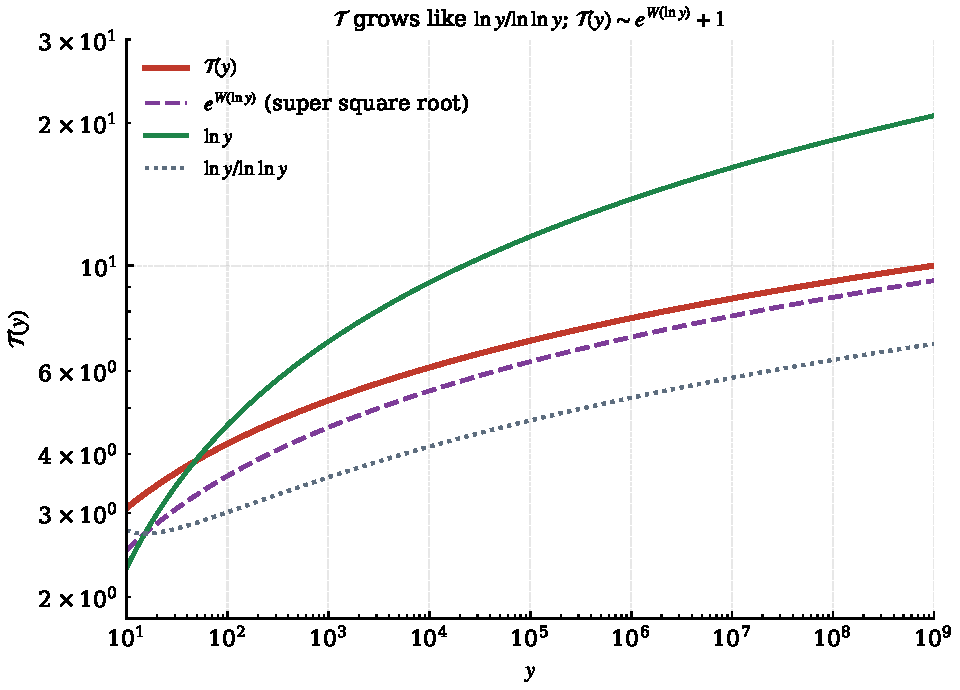
\includegraphics[width=0.78\textwidth]{figures/fig3_growth.pdf}
    \caption{Growth of $\Tah$ at large arguments (log-log scale):
    $\Tah(y)$ (solid red) runs just above the square super root
    $\ee^{W(\ln y)}$ (dashed purple), in accordance with the plus-one
    law \eqref{eq:asym-plusone}, and far below any power of $y$: its
    order is $\ln y/\ln\ln y$ (dotted curves).}
    \label{fig:growth}
\end{figure}

% =====================================================================
\section{Curiosities: integrals, a table of values, numerology, and
open problems}\label{sec:curiosities}
% =====================================================================

\subsection{Integrals}

Areas under $\Tah$ reduce, by the substitution $y = f(x)$, to areas
under $x^{x-1}$.

\begin{proposition}\label{prop:integrals}
\begin{align}
    \int_{0}^{1} \Tah(y) \dd y
    \;&=\; \alpha + \ln\alpha - \int_{1}^{\alpha} x^{x-1} \dd x
    \;=\; 1.432359924510\ldots, \label{eq:int1}\\
    \int_{-1}^{0} \bigl(1 - \Tah(y)\bigr) \dd y
    \;&=\; 1 - \beta + \ln\beta + \int_{\beta}^{1} x^{x-1} \dd x
    \;=\; 0.409721130782\ldots \label{eq:int2}
\end{align}
In \eqref{eq:int2} the integrand at the lower limit takes the value
$\beta^{\beta-1} = (1-\beta)/\beta = v$, the constant of
Theorem~\ref{thm:network}.
\end{proposition}

\begin{proof}
Substitute $y = f(x)$, $\dd y = f'(x)\dd x$. For
\eqref{eq:int1}: $\int_{0}^{1} \Tah(y) \dd y = \int_{1}^{\alpha}
x\, f'(x) \dd x = \bigl[x f(x)\bigr]_{1}^{\alpha} - \int_{1}^{\alpha}
f(x) \dd x = \alpha - \int_{1}^{\alpha}\bigl(x^{x-1} -
\tfrac1x\bigr)\dd x$. For \eqref{eq:int2}: $\int_{-1}^{0}
\bigl(1 - \Tah(y)\bigr)\dd y = \int_{\beta}^{1} (1-x) f'(x) \dd x
= \bigl[(1-x)f(x)\bigr]_{\beta}^{1} + \int_{\beta}^{1} f(x)\dd x
= (1-\beta) + \int_{\beta}^{1} x^{x-1}\dd x + \ln\beta$. The decimal
values were computed by high-precision quadrature and re-verified
through the right-hand sides.
\end{proof}

Neither $\int x^{x-1}$ nor any relative of it has a known closed
form; the classical neighbors are the two \emph{sophomore's dream}
integrals \cite{mathworld-sd},
$\int_{0}^{1} x^{-x}\dd x = \sum n^{n-1}/n!$ and
$\int_{0}^{1} x^{x} \dd x = \sum (-1)^{n+1} n^{-n}$, whose series
involve the very powers $n^{-n}$ that populate our parameters $b_n$.
Whether \eqref{eq:int1} admits an evaluation in terms of known
constants is Open Problem~\ref{op:integral}.

\subsection{A table of values}

For reference and numerical spot-checks we record
Table~\ref{tab:values}, computed to eighty significant digits and
truncated here; the exact entries are from
Proposition~\ref{prop:exactvalues} and
Theorem~\ref{thm:transcendence}, and every transcendental entry was
verified through its defining equation.

\begin{table}[t]
\centering
\small
\caption{Values of $\Tah$ at selected arguments. The entries at
$b \in \{0, \tfrac32\}$ are exact (Proposition~\ref{prop:exactvalues});
$\Tah(1) = \alpha$ and $\Tah(-1) = \beta$ are the constants of the
constellation.}
\label{tab:values}
\begin{tabular}{rll}
\toprule
$b$ & $\Tah(b)$ & remark \\
\midrule
$-10$    & $0.0000452971906610539$ & $\approx \ee^{-10}$ \\
$-5$     & $0.00622336542629749$  &  \\
$-2$     & $0.105721516538092434$ &  \\
$-3/2$   & $0.175410254005848625$ &  \\
$-1$     & $0.303659127029966051$ & $\beta$, A226568, transcendental \\
$-1/2$   & $0.556573703488657722$ &  \\
$0$      & $1$                    & exact; $=\varphi_0$ \\
$1/2$    & $1.45595925301034942$  &  \\
$1$      & $1.77677504009705470$  & $\alpha$, A124930, transcendental \\
$3/2$    & $2$                    & exact; $=\varphi_{3/2}$ \\
$2$      & $2.16575937062328429$  & partner of the root $x = -1$ \\
$\ee$     & $2.34459646238796334$ &  \\
$\pi$     & $2.42877946150189671$  &  \\
$5$      & $2.69536745976022816$  &  \\
$10$     & $3.07706224655857979$  &  \\
$100$    & $4.20694896031877337$  &  \\
$10^{6}$ & $7.74780160879762861$  &  \\
\bottomrule
\end{tabular}
\end{table}

\subsection{Numerology, debunked}

Constants as charismatic as $1.776775\ldots$ attract numerological
claims the way Tahawus attracted titanium prospectors. The
near-coincidence $\alpha \approx \sqrt{\pi}$ (they share two decimal
digits) dissolves under measurement:
\[
    \alpha - \sqrt{\pi} \;=\; 4.321189\ldots \times 10^{-3},
\]
a gap four thousand times wider than the precision to which $\alpha$
is known. A subtler trap, since it survives five digits, is
\[
    \alpha + \frac{1}{\alpha} - \bigl(\sqrt{\pi} + W(1)\bigr)
    \;=\; -4.6497 \times 10^{-6} ,
\]
and no doubt with a little effort one could manufacture coincidences
surviving eight. The theorem-level response is that
$\alpha$ is transcendental (Stanley; Corollary~\ref{cor:stanley}), so
\emph{no} identity expressing $\alpha$ through algebraic numbers can
hold exactly; identities mixing $\alpha$ with other transcendental
constants are not excluded by the theorem but are ruled out
numerically for every natural candidate we tested
($\alpha\beta = 0.5395339\ldots$, $\alpha + \beta = 2.0804341\ldots$,
$\alpha - \varphi = 0.1587410\ldots$, $1/\alpha = 0.5628174\ldots$,
none of them recognizable). The honest summary: the Tahawus constant
is a genuine constant, not a photograph of $\sqrt{\pi}$ wearing a
different hat.

\subsection{Open problems}

\begin{enumerate}[label=\textup{(\arabic*)}, leftmargin=2.2em]

\item\label{op:closedform} \textbf{No closed form.} We conjecture that
no finite expression built from the Lambert $W$ function---or from the
generalized Lambert functions of \cite{mezobaricz}---by composition,
arithmetic operations, and inversion solves the super-quadratic
$x^{x} = bx + 1$. The structural obstruction outlined in
Section~\ref{sec:background} (the unknown occurring as base, exponent,
and linearly) is not covered by any existing no-closed-form theorem
that we know of.

\item\label{op:complex-roots} \textbf{Complex roots.} How many complex
solutions does $z^{z} = z + 1$ have (per branch of the power)? By
Remark~\ref{rem:complex-roots} all of them are transcendental, but
even the count is open; nothing seems to be known about their
distribution.

\item\label{op:radius} \textbf{The radius, rigorously.} Prove that the
conjugate critical values $y_{c}, \overline{y_{c}}$ of
Subsection~\ref{subsec:radius} are the nearest singularities of the
principal branch of $\Tah$, making $R = 0.6526100\ldots$ a theorem.
The numerical evidence is strong (two independent methods, broad
critical-point sweep), but a proof requires control of all critical
values of $f$ in the disk of radius $R$.

\item\label{op:series} \textbf{The Maclaurin coefficients.} The
coefficients $d_{n}$ of \eqref{eq:maclaurin} are rational
($d_{3} = -\tfrac12$, $d_{6} = -\tfrac{49}{120},
\; d_{12} = \tfrac{62041117}{19958400}, \ldots$). Is there a closed
form, a hypergeometric-type characterization, or a generating function
for them? Is $d_{2} = 0$ the only vanishing coefficient? Do the
numerators and denominators appear in the OEIS?

\item\label{op:family} \textbf{The super-golden family.} For
$n \in \N$ let $\tau_{n}$ be the unique root of $x^{x} = x^{n} + 1$ in
$(n, n+1)$; then $\tau_{1} = \alpha$ and $\tau_{2} = \delta$, the
fixed point of Theorem~\ref{thm:fixedpoint}. The Gelfond--Schneider
step of Theorem~\ref{thm:transcendence} applies verbatim to every
$\tau_n$; what is missing is a uniform exclusion of rational roots.
Numerically $\tau_{n} = n + \bigl(n^{n}\ln n\bigr)^{-1}
\bigl(1 + o(1)\bigr)$ (already accurate to $4\%$ at $n = 3$): the
family approaches the integers super-exponentially fast. Is
$\tau_{n}$ transcendental for every $n$? We have not found
$\delta = \tau_{2}$ or any other $\tau_{n}$, $n \ge 2$, recorded in
the OEIS.

\item\label{op:tower-complex} \textbf{Complex dynamics of the
decremented tower.} Describe the Fatou/Julia dichotomy for
$z \mapsto \alpha^{z} - 1$ on the complex plane: the attracting fixed
point $0$, the repelling fixed point $\alpha$
(Theorem~\ref{thm:tower}), and the escaping set. For which bases
$a \in (1, \ee)$ does the boundary between the basin of $0$ and the
escaping set disconnect the plane?

\item\label{op:integral} \textbf{The integral.} Evaluate
$\int_{1}^{\alpha} x^{x-1}\dd x$ (equivalently
\eqref{eq:int1}) in terms of named constants or series, or prove that
no such expression exists in a reasonable class. The same question
for the moments $\int_{0}^{1} \Tah(y)^{k} \dd y$.

\end{enumerate}

The Tahawus function began life as a blog post's act of friendship
toward a beautiful unsolvable equation; we hope to have shown that it
repays systematic study. Every constant it touches---$\alpha$,
$\beta$, $v$, $\delta$---is transcendental, its graph threads between
$\ee^{y}$ and $1+y$ with third-order degeneracy at the origin, and
its inverse-functional structure ties the Lambert $W$ function, the
sophomore's dream, and the golden ratio into one small, coherent
constellation. The ghost town has a functioning mathematical namesake
at last.
